\documentclass[11pt,a4paper]{article}
\usepackage[margin=1in]{geometry}

\usepackage{tikz}
\usepackage{pgfplots}
\usepgfplotslibrary{groupplots} 
\usetikzlibrary{pgfplots.groupplots}
\usetikzlibrary{matrix,arrows,decorations.pathmorphing}
\usepackage{pgfplots,pgfplotstable}
\usepgfplotslibrary{fillbetween}
\usetikzlibrary{matrix,arrows,decorations.pathmorphing}


\usepackage{amssymb,amsthm}



\usepackage{amsmath}
\usepackage{enumerate}
\usepackage{epsfig}
\usepackage{bm}
\usepackage{verbatim}
\usepackage{graphicx}
\usepackage{hyperref}
\usepackage{xcolor}
\usepackage{algorithm}
\usepackage{algpseudocode}
\usepackage{float}


\usepackage{thmtools}
\declaretheoremstyle[%headfont=\normalfont
]{normalhead}
\declaretheorem[style=normalhead]{problem}
\declaretheorem[style=normalhead]{solution}

\DeclareMathOperator*{\argmin}{arg\,min}
\DeclareMathOperator*{\argmax}{arg\,max}

\usepackage{../rh_defs}

\newcommand\setG{\mc G}
\newcommand\vmu{\bm \mu}
\newcommand\mSigma{\bm \Sigma}

%\newcommand{\SHOWSOLUTION}[1]{}
\newcommand{\SHOWSOLUTION}[1]{#1}



\begin{document}

\center{\large \sc Deep Learning and Inverse Problems \\ Summer 2025}

Reinhard Heckel    
\center{ {\bf Chapter 4 exercises} 

Issued: Thursday May~6, 2025 \\
Due: Thursday May~13, 2025. \\[1em]

{\rule{\linewidth}{.2mm}}



\begin{problem}[Signal separation]
	
	Below is a question and the corresponding response from ChatGPT (generated with GPT4 in May 2023). Is the algorithm proposed by ChatGPT correct? If yes, can you help to answer how large the sparsity levels $s_1$ and $s_2$ can be for the algorithm to succeed? Provide references to results from the literature (e.g., from the book) in your answers. 
	
	\centering
	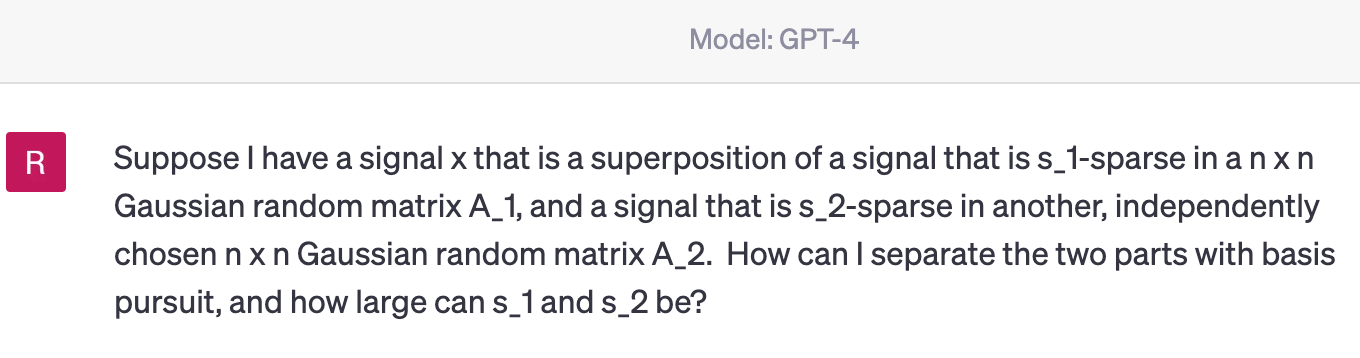
\includegraphics[width=140mm,scale=0.25]{./fig/chatGPT_prompt.png}
	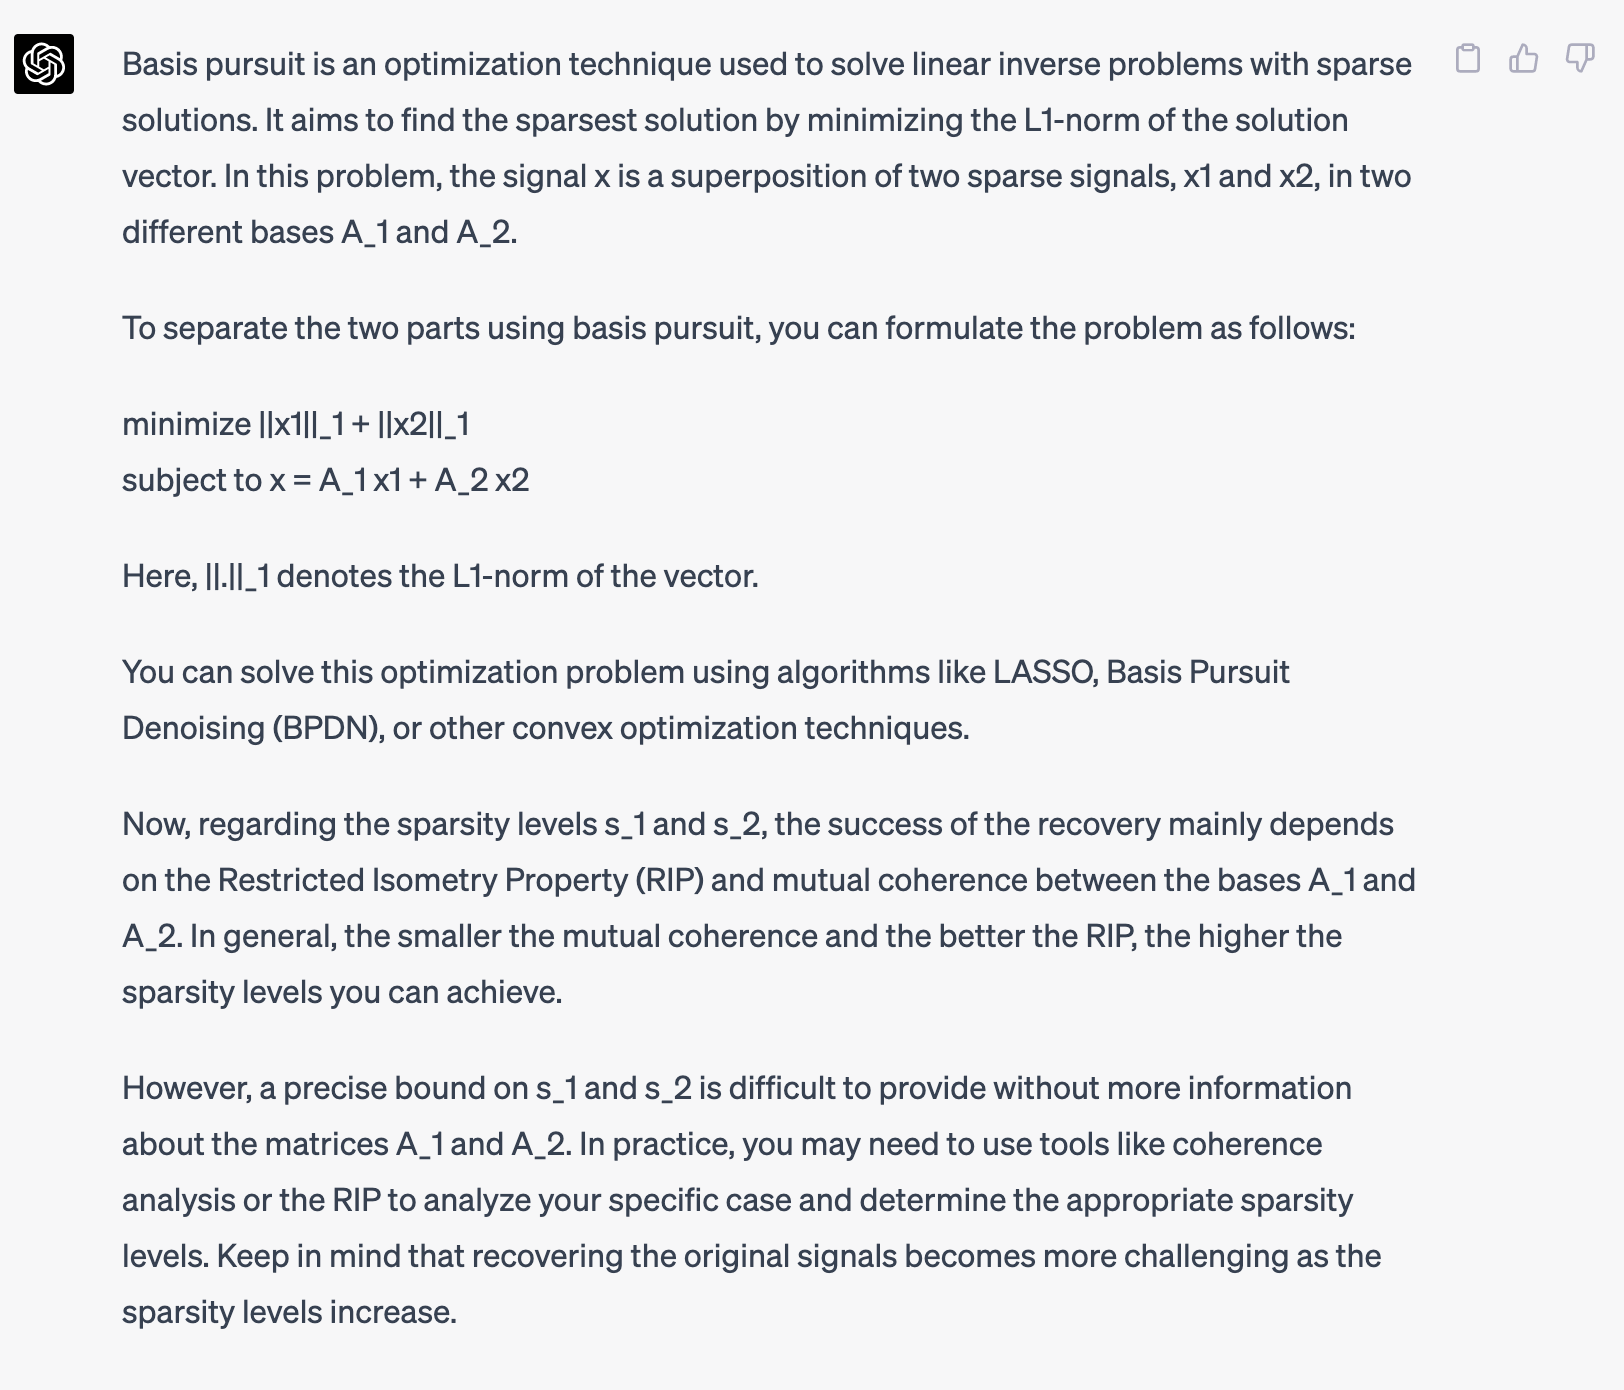
\includegraphics[width=140mm, scale=0.25]{./fig/chatGPT_answer.png}
\end{problem}

%%%


\problem[Compressive sensing with spikes and random vectors]{
In this problem we consider recovery of a signal that is sparse in the concatenation of the identity basis and a random basis, i.e., in the dictionary
\[
\mD = [\mB, \mI] \in \reals^{n\times 2n}.
\]
Here, $\mB \in \reals^{n\times n }$ is random Gaussian matrix, with entries iid $\mc N(0,1/n)$, and $\mI \in  \reals^{n\times n}$ contains the standard basis vectors, i.e., the $k$-th column of $\mI$ is the unit vector $\ve_k$ with $k$-th entry equal to one.
%Our goal is to recover the $s$-sparse vector $\vx$ from the measurement 
%\[
%\vy = \mD \vx.
%\]
\begin{enumerate}
\item 
First, we are given the measurement
\[
\vy = [\vb_0,\ve_0,\ldots,\ve_{n-1}] \vx,
\]
where $\vx$ is $s$-sparse. Furthermore, suppose the support set of $\vx$, i.e., the position of the non-zeros is known. How large can $s$ be such that recovery of every $s$-sparse vector from the corresponding measurement $\vy$ is possible, with probability one, and why?

\end{enumerate}

Next, we study recovery of $\vx$ from the measurement 
\[
\vy = \mD \vx. 
\]
Towards this goal, we first study the incoherence of the matrix $\mD$. Recall from class, that a matrix $\mA$ with unit norm columns is $\mu$-incoherent if $\mu$ is the smallest number such that for all pairs of columns $\va_i, \va_j$, $i\neq j $ of $\mA$, %\ym{smallest?}%
\[
\left|\innerprod{ \va_i }{ \va_j }  \right|
\leq
\mu.
\]
Also recall that for a Gaussian random variable $x \sim \mc N(0,1)$, we have that, for $\beta \geq \frac{1}{2\pi}$ that
\[
\PR{ x \geq \beta} \leq e^{-\beta^2 / 2}.
\]

\begin{enumerate}
\setcounter{enumi}{1}
%%%
\item 
What is the distribution of $\innerprod{\ve_i}{\vb_j}$, and given this result, what is bound on the probability that the absolute values of this random variable exceeds a constant $\beta'$ %\ym{$\geq \frac{1}{2\pi}$?} ?
?

\item Building on the result from the previous part, what is the coherence parameter of the matrix $\mD$, with high probability (say with probability at least $1-\delta$, where $\delta >0$ is a parameter)? 
Since $\norm[2]{\vb_i} \approx 1$, with high probability, you can assume $\norm[2]{\vb_i} = 1$ for simplicity.




%
\item
Recall from class that provided a matrix $\mA$ is $\mu$-incoherent, and $\vx$ is $s$-sparse with $s < \frac{1}{2\mu}$, then $\ell_1$-minimization provably recovers the vector $\vx$ from the measurements $\vy = \mA \vx$.
Based on this result, what is the maximum sparsity under which recovery with $\ell_1$-minimization provably succeeds?
Is this result pessimistic, i.e., is there a matrix that allows the sparsity $s$ to be significantly larger, if yes, specify that matrix and specify what the allowed level of sparsity is. 
\end{enumerate}

}


\end{document}

